%% main.tex
%%%%%%%%%%%%%%%%%%%%%%%%%%%%%%%%%%%%%%%%%%%%%%%%%%%%%%%%%%%%%%%%%%%%%%%%%%%%%%%%
\documentclass[
    fontsize=10pt,
    twoside=true,
    numbers=noenddot
]{cls/phdbyphd}

\usepackage[english]{babel}
\usepackage[english=british]{csquotes}
\usepackage{amsmath}
\usepackage{textcomp}
\usepackage{fontawesome}

\usepackage{styles/phdbibliobyphd}
\addbibresource{main.bib}

\graphicspath{{imgs/}{./}}
\newcommand\home{./}  % for path adjustments 

\makeindex[columns=3, title=Alphabetical Index, intoc]
%\makeglossaries
%\makenomenclature

%%%%%%%%%%%%%%%%%%%%%%%%%%%%%%%%%%%%%%%%%%%%%%%%%%%%%%%%%%%%%%%%%%%%%%%%%%%%%%%%
\begin{document}

\pagenumbering{Alph}

%%%%%%%%%%%%%%%%%%%%%%%%%%%%%%%%%%%%%%%%%%%%%%%%%%%%%%%%%%%%%%%%%%%%%%%%%%%%%%%%
\titlehead{Master of Science in Engineering with Specialisation in Data Science}

\subject{Master Thesis}
\title[On Improving Pattern Recognition in Deep Learning Systems through Self-Organization]{
    On Improving Pattern Recognition in Deep Learning Systems through Self-Organization
}
\subtitle{Incorporating Findings from Neuroscience about Brain Functionality into Modern Deep Learning Architectures}

\author[Pascal Sager]{Pascal Sager}
\date{\today}

\publishers{Zurich University of Applied Sciences}

%%%%%%%%%%%%%%%%%%%%%%%%%%%%%%%%%%%%%%%%%%%%%%%%%%%%%%%%%%%%%%%%%%%%%%%%%%%%%%%%
\frontmatter
\setchapterstyle{plain}

%%%%%%%%%%%%%%%%%%%%%%%%%%%%%%%%%%%%%%%%%%%%%%%%%%%%%%%%%%%%%%%%%%%%%%%%%%%%%%%%
\dedication{
	Dedicated to the dedicated.\\
	\flushright -- Pascal Sager
}

%%%%%%%%%%%%%%%%%%%%%%%%%%%%%%%%%%%%%%%%%%%%%%%%%%%%%%%%%%%%%%%%%%%%%%%%%%%%%%%%
\KOMAoptions{twoside=semi}
\maketitle
% \KOMAoptions{twoside=false}
%%%%%%%%%%%%%%%%%%%%%%%%%%%%%%%%%%%%%%%%%%%%%%%%%%%%%%%%%%%%%%%%%%%%%%%%%%%%%%%%
% Inspirational quote
\begin{prequote}[20pt]{Geoffrey Hinton, University of Toronto, 2017.}
    "Max Planck said, ‘Science progresses one funeral at a time.’\\
    The future depends on some graduate student who is deeply\\
    suspicious of everything I have said."\\

\end{prequote}

%%%%%%%%%%%%%%%%%%%%%%%%%%%%%%%%%%%%%%%%%%%%%%%%%%%%%%%%%%%%%%%%%%%%%%%%%%%%%%%%
\chapter*{Zusammenfassung}
\addcontentsline{toc}{chapter}{Zusammenfassung}
    Deep Learning Systeme haben in den letzten Jahren beeindruckene Resultate erzielt und können unter anderem mit hoher Qualität Texte übersetzen, Unterhaltungen führen oder Bilder generieren. Diese Systeme werden typischerweise mit Backpropagation of Error über sämtliche Netzwerklayer hinweg als ein grosses System trainiert. Dieser Prozess ist zwar für spezifische Task wie Klassifizierung sehr effizient, ist aber neurowissenschaftlich nicht plausibel und hat verschiedenste Schwächen wie fehlende Robustheit sowie Interpretierbarkeit und nicht die Fähigkeit kausale Schlussfolgerungen zu ziehen.

In dieser Thesis werden neurowissenschaftliche Erkenntnisse identifiziert, die für die Intelligenz von Lebewesen wie dem Mensch elementar sind und auf Deep Learning Systeme übertragen. Der Fokus liegt dabei auf dem visuellen Cortex als biologische Inspirationsquelle und Deep Learning Architekturen zur Bildverarbeitung als Zielsystem. Neurowissenschaftliche Erkenntnisse beziehen sich auf biologische Neuronen, welche sich gegenseitig durch zeitabhängige Spannungsspitzen gegenseitig anregen oder hemmen. Deep Learning Systeme hingegen haben keine Zeitdynamik und haben Aktivierungen basierend auf Fliesskommazahlen anstelle von Stromimpulsen. Folglich besteht ein grosser Beitrag dieser Arbeit darin die neurowissenschaftlichen Erkenntnisse in den Kontext von Deep Learning zu übertragen.

Die abgeleiteten Erkenntnisse werden in Form von zwei konkreten Modellen implementiert. Dabei besteht darin, neue Architekturideen zu demonstrieren und nicht irgendwelche Metriken von Benchmark-Datensätzen zu überbieten. Zudem orientieren sich die vorgeschlagenen Architekturen nahe am bewährten Deep Learning Framework und sind nicht als biologisch plausible Systeme zu verstehen. Konkret wird ein Modell mit vertikaler und ein Modell mit horizontaler Selbst-Organisation vorgeschlagen. Das Modell mit vertikaler Selbst-Organisation optimiert jedes Modell-Layer separat. Dabei werden neue Konzepte vorgestellt, die es erlauben alle Layer gleichzeitig zu trainieren und trotzdem hierarchische Features über die Layer hinweg zu erlernen. Das zweite Modell mit horizontaler Selbst-Organisation teilt die Eingabedaten in kleinere Einheiten auf und verteilt diese auf unabhängig trainierte Modelle. Dabei sieht jedes Modell nur ein Teil der Eingabedaten und ist auf eine lokale Interaktion mit seinen Nachbarmodellen angewiesen, um eine passende Bildrepräsentation abzuleiten.

TODO: Schlussfolgerung / Erkenntnisse sobald Experimente abgeschlossen sind.
    
\chapter*{Abstract}
\addcontentsline{toc}{chapter}{Abstract}
    In the past decade, deep learning has established itself as state-of-the-art technology in various automatic image analysis tasks.
Despite impressive results, this technology has several limitations, notably its limited robustness to noise, constrained transformation invariance during object recognition and reliance on a substantial amount of training data.
Although many research approaches strive to mitigate these limitations, they often limit themselves to reducing the symptoms by, for example, augmenting data, thereby sidestepping the underlying cause, which is rooted in the foundational learning paradigm of deep neural networks.

Conversely, the human does not suffer from these limitations, partly due to its non-sequential processing of extracted image features and its ability to perceive visual scenes holistically, i.e. interpret it as more than the sum of its part, as outlined by Gestalt psychology.
Building upon these insights, this thesis proposes a novel image-processing framework strongly oriented towards the functioning of the human brain.
Accordingly, a significant part of this thesis is devoted to identifying and interpreting neuroscientific findings.
These findings are analysed and translated into a computational framework, assigning distinct roles to each framework component and clarifying their congruence with biological learning.

The framework consists of three components: The sensor system \emph{S0},  responsible for extracting low-level features from the images; the feature-building stage \emph{S1}, which uses lateral (intra-layer) connections to form neuron groups, so-called net fragments,  fostering mutual support to stabilise known patterns; the prototype stage \emph{S2}, which maps the formed net fragments to object prototypes using projection fibres and provides feedback to \emph{S1}.
This iterative projection process lasts until consistency is achieved at every point in the network, i.e. until cells and synapses have reached a stable attractor state.
Notably, all learning processes are thereby limited to self-organisation and local interaction. This is a clear distinction from conventional neural networks that typically enforce consistency at a single point in the network between a prediction and a teaching signal, utilising a global error correction algorithm such as backpropagation of error.

While prior research has demonstrated the efficiency of projection fibres, implementing net fragments still needs to be explored.
Consequently, this thesis explores the implementation of this component in detail and discusses it by conducting experiments with a simple dataset based on straight lines.

The experimental findings show that lateral connections trained with Hebbian learning can effectively facilitate cell support.
The network exhibits significant robustness using cell support and can deactivate up to $91.7\%$ of unwanted cell activity triggered by noise signals. Furthermore, lateral support can restore discontinuous lines, demonstrating the network's ability to deal with occluded objects. With a range of lateral connections of $11$ pixels, interruptions of up to $8$ pixels can be reconstructed, and with additional feedback from \emph{S2}, even interruptions of up to $20$ pixels can be restored. The proposed framework has the potential to address several weaknesses of conventional neural networks and presents a promising alternative to current image processing algorithms.

%%%%%%%%%%%%%%%%%%%%%%%%%%%%%%%%%%%%%%%%%%%%%%%%%%%%%%%%%%%%%%%%%%%%%%%%%%%%%%%%
\chapter*{Preface}
\addcontentsline{toc}{chapter}{Preface}
    \small
This thesis is the last hurdle before I will hold the title ``Master of Science''.
To me, science means the systematic analysis of the real or virtual world through observations and experiments as well as the further development of existing technology. 
I am lucky enough to be able to apply the knowledge and methodologies I learned during my studies to research projects at the Centre for Artificial Intelligence (CAI) of the Zurich University of Applied Sciences (ZHAW).
I was mentored and supported during my studies by Prof. Dr. Thilo Stadelmann.
He uses to say (also in accordance with his \href{https://stdm.github.io/Great-methodology-delivers-great-theses/}{blog-post}) ``Great methodology delivers great theses''.
It is always desirable to have an excellent outcome such as a system that can execute a task and thereby achieves or even overcomes state-of-the-art performance.
However, in my opinion, it is equally or even more important to reason why and how something works, to justify choices, and to show limitations.
I wrote my Thesis with these thoughts in mind and hope that the readers are able to follow my reasoning.

In the Introduction section, the work is motivated and in the subsequent chapter the fundamentals of Deep Learning and its limitations is described.
Afterwards, it is motivated why methodologies inspired by neuroscience could overcome these limitations.
This thesis aims at a target audience with a background in Deep Learning.
Consequently, the concepts of Deep Learning are only roughly described.
Since Neurocomputing may be rather unknown to the target audience, a more extensive overview about this field is given.

I would like to thank a couple of colleagues and friends.
First I think of my mentor Prof. Dr. Thilo Stadelmann who got me excited about AI years ago and later introduced me to research.
He always encouraged creative ideas and helped to link different research areas to address problems with methodologies from other fields.
Thanks to his support, help, and guidance, I have grown personally as well as professionally.
Further thanks go to Dr. Jan Deriu. 
Especially at the beginning of my thesis, he steered my thoughts in one direction.
His unconventional thinking has led to the questioning of many methods that have stood the test of time for decades (this was also the inspiration for Geoffrey Hinton's quote on the page before, although I wouldn't presume to say that this thesis will change the future).
To Prof. Dr. Christoph von der Malsburg for his seemingly endless patience in introducing me to neuroscience.
He can build the bridge between the two diverging fields of Deep Learning and Neuroscience, inspires to think outside the box.

The biggest thanks, however, goes to my family, who made this journey possible for me.
My parents, who supported and encouraged me in every way.
My younger brother who inspired me to study.
My wife and son, who have been understanding and supportive and have always been the perfect counterbalance to the daily routine of studying.
Without the support of my family, I would never have been able to embark on this academic path.
\normalsize


%%%%%%%%%%%%%%%%%%%%%%%%%%%%%%%%%%%%%%%%%%%%%%%%%%%%%%%%%%%%%%%%%%%%%%%%%%%%%%%%
% TOC / LOF / LOT
\begingroup

    \setlength{\textheight}{23cm}
    \etocstandarddisplaystyle
    \etocstandardlines

    \tableofcontents

    \listoffigures

    \let\cleardoublepage\bigskip
    \let\clearpage\bigskip

    \listoftables

    %\afterpage{\blankpage}

\endgroup

%\KOMAoptions{twoside=false}

%%%%%%%%%%%%%%%%%%%%%%%%%%%%%%%%%%%%%%%%%%%%%%%%%%%%%%%%%%%%%%%%%%%%%%%%%%%%%%%%
%%%%%%%%%%%%%%%%%%%%%%%%%%%%%%%%%%%%%%%%%%%%%%%%%%%%%%%%%%%%%%%%%%%%%%%%%%%%%%%%
\mainmatter
\setchapterstyle{phdbyphd}

% \afterpage{\blankpage}\addtocounter{page}{-1}

\setchapterpreamble[u]{\margintoc}
\chapter{Introduction}\chlbl{intro}
%% intro.tex
Humanity has always tried to simplify its life through technological progress.
The computer has shaped progress in every field imaginable in the last hundred years. 
In fact, it has been so successful that it has spawned its own scientific discipline, computer science.
Nowadays, it is impossible to imagine life without computers: almost every household and company owns at least one.
Computers facilitate various tasks, from communication to the acquisition of knowledge.
For all these tasks, software developers have created appropriate programs.
Software development is the process of writing a script with a programming language to specify how the computer should behave for a given input.
Simply put: A software program tells the computer what to do if the user enters a command.
Writing software can be done easily if the tasks are clearly defined and can be described precisely.
However, there exist tasks that are almost impossible to program, such as writing a script that detects cats in images because we cannot describe to a computer how a cat looks precisely\sidenote{at least not on a pixel-level basis so that we can compare a given image with our description}.

Therefore, scientists came up with the idea to not just program such tasks but to let the computer learn them.
Machine learning (ML) algorithms can learn and adapt without following explicit instructions such as program code.
Instead, they use statistical models to analyse data, find patterns, and make predictions.
Machine learning has become an indispensable part of our everyday lives.
For example, we use it for machine translation, transport and logistics organisation, product recommendations, fraud detection, self-driving cars, unlocking smartphones, improving video games, speech recognition, and much more.
A sub-branch of machine learning is deep learning (DL) which achieved awe-inspiring results in the last decade and is considered \emph{the} state-of-the-art technology for many of the aforementioned tasks.

Even though this technology works very well for many tasks, such models have some crucial flaws by definition (c.f. \secref{limitationsDL}), which cannot be resolved in the current DL framework.
One of the godfathers of deep learning is Turing Award\sidenote{the Turing Award is recognized as the highest academic award in computer science and sometimes also called the ``Nobel Prize of Computing''} winner Geoffrey Hinton. 
Especially his contribution to learning with backpropagation of error (c.f. \secref{ann}) has created the foundation for modern deep learning systems.
More than 30 years later, Hinton says he is ``deeply suspicious'' about end-to-end backpropagation of error. In his opinion, we have to ``throw it all away and start again'' to improve current systems fundamentally \sidecite{axios_hinton}.
This seems rather extreme considering what DL systems have achieved.
However, it also shows that the current learning algorithm of such systems has serious flaws.

Some of the most critical limitations of deep learning systems are listed in \secref{limitationsDL}.
This thesis addresses these problems by exploring different architectures inspired by findings from neuroscience\sidenote{the field of neuroscience studies how the human nervous system and especially the brain works}.
The inspiration is drawn from neuroscience, as the human brain does not have these problems. Thus, incorporating findings from neuroscience into the deep learning framework might help overcome some of the current limitations.
In this thesis, the ``Theory of Natural Intelligence'' by von der Malsburg et al. \sidecite{von_der_Malsburg_Stadelmann_Grewe_2022} in particular is used as inspirational source.
The aforementioned theory focuses on the visual processing in the human brain, and consequently, deep learning architectures for image processing are examined.
Thereby, the main focus of this thesis is on \emph{finding new principles} of deep learning architectures rather than on achieving state-of-the-art performance in terms of accuracy or f-score on existing benchmarking datasets.

The thesis differs from neurocomputing\sidenote{neurocomputing is a sub-field of neuroscience that deals with the implementation of learning algorithms with a high degree of biological plausibility} in the sense that the architectures investigated are still closely related to the DL framework and, for example, do not use time-dynamic signals. 
For the completeness of this thesis, an overview of neurocomputing is given in \secref{neurocomputing}.
However, since these neurocomputing algorithms have not (yet) become established in practical applications, they are not investigated in this thesis.
Thus, the thesis is strongly oriented along the field of deep learning and focuses on incorporating neuroscience findings in the deep learning framework, while natural plausibility is considered less important.


%Mankind is often inspired by nature when it comes to developing novel systems.
%The development of artificial intelligence (AI) and Deep Learning has been strongly influenced by, according to our perception, one of (if not the) most intelligent systems on planet Earth, the human brain.
%The brain is studied by the scientific field of neuroscience\sidenote{there exist many additional (sub-)fields studying the brain such as cognitive science, cognitive psychology, neurology, and neuropsychology}.
%From neuroscience or related fields come various insights on how the human nervous system and especially the brain works.
%Much of this knowledge has been gained through observations and experiments on humans or other living creatures.
%Often these findings are only what can be measured from the outside, the real core, the mechanism that causes intelligence, remains unknown.
%
%While Deep Learning is clearly inspired by the insights of Neuroscience, the two fields have little in common in their present form.
%The implementation of neuroscientific findings has emerged as a subfield in its own right, called Neurocomputing (c.f. Section \secref{neurocomputing}).
%In general, neurocomputing is closer related to the functionality of the human brain than Deep Learning.
%Neurocomputing has produced many promising algorithms that can overcome some weaknesses faced by deep learning systems. 
%Although neurocomputing has also achieved significant breakthroughs, most systems used in everyday life are still based on the principle of Deep Learning.


%\section{Motivation}\seclbl{motivation}
%One of the main challenges of today's AI systems is the processing of visual information.
%Visual perception is fundamentally the task of finding a suitable interpretation of a given scene.
%A scene typically consists of objects that interact with each other.
%Identifying these objects and their relationship among each other is implemented by algorithms as a non-deterministic search problem, i.e. algorithms try to identify the object within a scene.
%State-of-the-art algorithms for image processing are often based on deep learning.
%Despite the fact that deep learning has achieved incredible performance on a variety of tasks such as object recognition it is still questionable whether the current methodology is enough to achieve real (or at least more advanced) intelligence (c.f. Section \secref*{limitationsDL}).
%Algorithms from the field of neurocomputing (c.f. Section \secref*{neurocomputing}), which are more closely oriented to the findings from the field of neuroscience, can be considered as a complement to deep learning.
%However, even tough algorithms from the field of neurocomputing have interesting properties, they usually do not perform as good as deep learning according to the evaluation metrics used and often work on specific or small data only.

%Thus, various algorithms exist to solve the non-deterministic problem of finding an appropriate interpretation of a visual scene, but they have significant shortcomings.
%Interestingly, the problem of generating a scene\sidenote{the opposite task than finding an interpretation of a scene} from a clear description is deterministic.
%Computer graphics deals with the problem to generate images with the aid of computers.
%Nowadays, such systems are able to render photorealistic images based on descriptions.
%For example, video games are essentially programs that generate scenes consisting of multiple objects such as people, weapons, buildings, or vehicles based on program code.
%For each of these objects, skeletons are usually pre-defined and during rendering transformed (i.e. their size, rotation, distortion and positioning are adjusted) as well as properly illuminated (raytracing).
%This allows to generate an infinite number of scenes from a predefined set of skeletons and transformations.
%Essential in this process seems the separation between objects and object transformation.
%Therefore, incorporating these insights into current algorithms for the interpretation of visual scenes seems promising and could lead to significant improvements.
%More precisely, identifying objects and their transformations separately in preception systems in order to recognise objects independently of their transformations could improve visual scene interpretation.


%\section{Terminology}\seclbl{terminology}


\section{Contribution}
This thesis makes the following contributions:
\begin{itemize}
	\item First, the basics of deep learning and neurocomputing are described in detail. Together with the related work, this provides a survey of the most important work that deals with improving learning generally.
	\item Second, promising concepts from the neuroscience literature that may be necessary for more intelligent systems are identified, and suggestions are made on integrating these concepts into modern DL frameworks.
	\item Third, two concrete DL architectures that use such neuroscience-inspired concepts are presented, and their strengths and weaknesses are analysed in detail.
	\item Fourth, this work provides an intuition of which concepts currently little used in DL settings seem promising and recommends future research directions.
\end{itemize}


\section{Organisation of Thesis}\seclbl{org_thesis}
The remainder of the thesis is organised as follows: In \chref{fundamentals}, the fundamentals of deep learning and neurocomputing are explained in detail.
Experts may skip this chapter; especially the second section on neurocomputing can optionally be omitted, as it is not fundamental for understanding this thesis, but only intended for interested readers or those who want to get a better overview of the field.
\chref{rel_work} introduces the related work. Next, \chref{neuro_concepts} identifies promising findings from neuroscience that might help to improve current deep learning systems. Furthermore, it is proposed how these neuroscientific concepts could be implemented in a deep learning setting.
In \chref{vertical_self_org} and \chref{horizontal_self_org}, two different architectures incorporating these concepts are presented. Finally, in \chref{future_work}, future work is described, and some insights and intuitions of the author are given about which neuroscience concepts seem promising and which do not, and what the next steps for developing more intelligent systems could be.





\chapter{Motivation}\chlbl{motivation}
%% motivation.tex
Despite the fact that Deep Learning has achieved incredible performance on a variety of tasks it is still questionable whether the current methodology is enough to achieve real (or at least more advanced) intelligence (c.f. Section \secref*{limitationsDL}).
Many of the current limitations are tackled by approaches from the field of neurocomputing (c.f. Section \secref*{neurocomputing}).
Although many of the methods cannot yet compete with current DL models or work only on small data sets, these methods have shown promising results.
The neurocomputing methods are inspired by neuroscience (the study of the nervous system including the brain, spinal cord, and peripheral nervous system).
Neuroscience provides a source of inspiration for AI algorithms, independent of mathematical models.
Recently, von der Malsburg et al. \sidecite{von_der_Malsburg_Stadelmann_Grewe_2022} have published their hypothesis about the key building blocks for a system with general intelligence.
They point out that building self-organizing sub-networks during training may be one of the keys to fundamentally improve current systems.
Lehmann \sidecite{lehmann} worked on incorporating a few of these ideas and principles into a DL framework.
He proposes a laterally connected layer (LCL), a layer that forms lateral intra-layer connections based on Hebbian learning.
These connections are formed during training based on the input.
He shows that the LCL layer increases robustness on the popular MNIST dataset.
However, he also points out potential for improvement of the LCL layers.

Von der Malsburg et al. \cite{von_der_Malsburg_Stadelmann_Grewe_2022} propose several concepts how current problems in ANNs can be tackled.
They present systematically sound theoretical foundations, but neither the formulation of a mathematical model nor the translation of their ideas into a concrete application were in the scope of their work.
Specifically, we do the following...

TODO...





















\chapter{Related Work}\chlbl{rel_work}
%% related_work.tex

\section{Natural Intelligence}\seclbl{natural_intelligence}
This thesis is inspired by the work ''A Theory of Natural Intelligence` from von der Malsburg et al. \sidecite{von_der_Malsburg_Stadelmann_Grewe_2022}.
Therefore, we dedicate this section to summarize their work in detail.

According \cite{von_der_Malsburg_Stadelmann_Grewe_2022}, the process of learning is influenced by ``nature'', ``nurture'', and ``emergence''\sidenote{nature refers to the influence of genes and evolution, nurture to the influence of experience and education}.
They point out that human genome (as of nature) only contain 1GB of information \sidecite{hbcrd} and humans only absorb a few GB into permanent memory over a lifetime (as of nurture) but it requires about 1PB to describe the connectivity in human brain.
Therefore, it is important to distinguish the amount of information to describe a structure from the amount of information needed to generate it.
Similar, nature and nurture only require a few GB to construct, respectively instruct the entire human brain.
Therefore, they argue that the human brain must be highly structured (i.e. nature and nurture ``generate'' the human brain by selecting from a set pre-structured patterns).
The authors call the process of generating the highly structured network in the human brain the ``Kolmogorov \sidecite{Kolmogorov_1998} Algorithm of the Brain''\sidenote{as the Kolmogorov complexity describes the number of bits required by the shortest algorithm that can generate the structure}.
Network self-organization is the only mechanism that has not yet been disproved by experiments as the brains Kolmogorov algorithm \sidecite{Willshaw_VonDerMalsburg_1976, Willshaw_VonDerMalsburg_1979}.
This mechanism loops between activity and connectivity, with activity acting back on connectivity through synaptic plasticity until a steady state, called an attractor network, is reached.
The consistency property of an attractor network means that a network has many alternative signal pathways between pairs of neurons \sidecite{Malsburg_1987}.
Thus, the brain develops as an overlay of attractor networks called net-fragments \sidecite{vonderMalsburg_2018}.
Net-fragments consist of small sets of neurons, whereby each neuron can be part of several net fragments.
The network self-organization has to start from an already established coarse global structure which is improved in a coarse-to-fine manner to avoid being caught in a local optima.

Also, von der Malsburg et al. \cite{von_der_Malsburg_Stadelmann_Grewe_2022} discuss scene representation (i.e. how a scene is represented in the brain) even tough they point out that this is a contested concept \sidecite{freeman1990representations}.
Scene representation is a organization framework to put abstract interpretation of scene layouts, elements, potential actions, and emotional responses in relation.
The details are not rendered as in photographic images but the framework supports the detailed reconstructions of narrow sectors of the scene.
The basic goal if learning is to integrate a behavioral schema into the flow of scene representations.
They propose the hypothesis that the network structure resulting from self-organization together with the neural activation in the framework of scene representation are the inductive bias that tunes the brain to the natural environment.

Finally, they discuss how net fragments can be used to implement such structures and processes using vision as an example.
They point out that a neuron is grouped in one or multiple net fragments through network self-organization.
The net fragments can be considered as filters that detect previously seen patterns in the visual input signal.
An object is represented by multiple net fragments, where each fragment responds to the surface of that object and has shared neurons and connections with other net fragments representing that object.
Thus, net fragments render the topological structure of the surfaces that dominate the environment.
Von der Malsburg et al. \cite{von_der_Malsburg_Stadelmann_Grewe_2022} propose that net fragments represent shape primitives which can adapt to the shape of actual objects\sidenote{adapt in spite of metric deformations, depth rotation, and position}.
Shifter circuits are one possible implementation of networks that enable invariant responses to the position- and shape-variant representations \sidecite{Arathorn_2002, Olshausen1995}.
They are composed of net-fragments that can be formed by network self-organization \sidecite{Fernandes_vonderMalsburg_2015}.
Ref. \cite{von_der_Malsburg_Stadelmann_Grewe_2022} also argue that net fragments are the compositional data structure used by the brain.
A hierarchy of features may be represented by nested net fragments of different size.
Complex objects, such as mental constructs, can thus be seen as larger net fragments composed as mergers of pre-existing smaller net fragments.


\section{Self-Organization}\seclbl{self_org_related}
%% THIS WAS MOVED TO INTRO
%The human brain is self-organizing \sidecite{kelso1995dynamic}.
%Self-organization is the process by which systems consisting of many units spontaneously acquire their structure or function without interference from a external agent or system.
%The absence of a central control unit allow self-organizing systems to quickly adjust to new environmental conditions.
%Additionally, such systems have in-built redundancy with a high degree of robustness as they  are made of many simpler individual units.
%These individual units can even fail without the overall system breaking down.
%Dresp \sidecite{Dresp2020SevenPO} describes seven clearly identified properties of self-organization in the human brain: (i) modular connectivity, (ii) unsupervised learning, (iii) adaptive ability, (iv) functional resiliency, (v) functional plasticity, (vi) from-local-to-global functional organization, and (vii) dynamic system growth.

%Before summarizing the literature specific to self-organization of neural networks, the general literature on self-organization with a focus on deep learning is described in the following.
%Many of these fundamental algorithms for self-organization serve as inspiration for how ANNs can be designed to be self-organizing.

In nature, groups of millions units that solve complex tasks by using only local interactions can be observed.
For example, ants can navigate difficult terrain with a local pheromone-based communication and thus form a collective type of intelligence.
Such observations inspired researchers to build algorithms which are based on local communication and self-organization, for example ant colony optimization algorithms \sidecite{dorigo1997ant}.
DeepSwarm \sidecite{Byla_Pang_2020} is a neural architecture search method that uses this algorithm to search for the best neural architecture.
This methods achieves competitive performance on rather small datasets such as MNIST, Fashion-MNIST, and CIFAR-10.

%Robotic is another research area that uses ideas from collective intelligence such as self-assembly or self-organization.
%For example, swarm systems consist of multiple robots that work together to solve complex tasks \sidecite{Hamann_2018}.
%A famous example of self-assembling robots was presented in 2014 by Rubenstein et al. \sidecite{Rubenstein_Cornejo_Nagpal_2014}.
%They teach kilobots\sidenote{kilobots are 3.3cm tall low-cost swarm robots developed at Harvard University} to self-assemble into target shapes such as letters or stars solely based on local communication between robots.
%However, the kilobots still rely on hand-crafted algorithms to determine their position in the global coordinate system.

%TODO: Write more about swarm intelligence or delete thie paragraph above (does not really fit in here....)

Cellular Automata mimic developmental processes in multi-cell organisms.
They contain a grid of similar cells with an internal state which is updated periodically.
The transition from a given state to a subsequent state is defined by some update rules.
During an update, cells are only allowed to communicate with the neighbouring cells.
Thus, self-organization is enforced by the definition of the update rules.
Such automata can be used to study biological pattern formations \sidecite{Wolfram1984} or physical systems \sidecite{VICHNIAC198496}.
Neural Cellular Automata \sidecite{Wulff1992LearningCA} use neural networks to learn the update rule.
The input in such a neural network is the state of a given cell and its neighbours, the output the subsequent cell state.
Usually, the same network is applied to all cells.
In this case, a fully connected neural network which is applied to each cell and its local neighbours can be reformulated as a CNN\sidecite{PhysRevE}.
NCAs can be trained efficiently with gradient descent to grow given 2D patterns such as images\sidecite{48963, Mordvintsev_Randazzo_Fouts_2022}.
These images are grown through self-organisation (i.e. the pixels pick a color based on the color of neighboring pixels) and are surprisingly resistant to damage.
For example, large parts of the images can be removed and the system is able to rebuild these pixels\sidenote{a demo of this regeneration process is available at \cite{NCAs_distill}}.
However, the aforementioned approaches can only grow the pattern they were trained on.
A recent method called Variational Neural Cellular Automata \sidecite{Palm_GonDuque_Sudhakaran_Risi_2022} use an NCA as decoder of a Variational Autoencoder \sidecite{Kingma_Welling_2014}.
This probabilistic generative model can grow a large variety of images from a given input encoded in a vector format.
However, there is still a big gap in performance compared to state-of-the-art generative models.
Besides growing 2D patterns, NCAs can also create 3D patterns such as buildings in the popular video game Minecraft by utilizing 3D CNNs \sidecite{Sudhakaran_Grbic_Li_Katona_Najarro_Glanois_Risi_2021} or generate structures with specific function such as simulated robots able to locomote\sidecite{Horibe_Walker_Risi_2021}.
Moreover, self-assembling approaches based on NCAs are not restricted to grid-structures.
NCAs can be generalized to graph neural networks \sidecite{Grattarola_Livi_Alippi_2021}.
Graph cellular automata (GCA) use graph neural networks \sidecite{Zhou_Cui_Hu_Zhang_Yang_Liu_Wang_Li_Sun_2021} instead of CNNs to learn the state transition rules and can thus deal with more complex pattern structures than just 2D and 3D grids.
The process of growing images from cells of an NCA can also be inverted.
Randazzo et al. \sidecite{randazzo2020self_classifying} propose to use NCA to classify given structures such as images.
They apply the same network to each pixel and its neighbours of an image.
In an iterative process based on local communication, the image fragments then agree on which object they represent.
NCAs can even be used to control reinforcement learning (RL) agents.
Variengien et al. \sidecite{Variengien_Nichele_Glover_Pontes_Filho_2021} use the observations of the environment as state of the NCA, the subsequent state predicted by the NCA are used as Q-value estimates of a deep Q-learning algorithm \sidecite{Mnih_Kavukcuoglu_Silver_Graves_Antonoglou_Wierstra_Riedmiller_2013}.

Self-organization can not only be used to generate structures but also to optimize the weights of a neural networks over the agents lifetime.
For example, a Hebbian learning rule for meta-learning can be used to self-organize the weights of a RL agent over his lifetime\sidecite{NEURIPS2020_ee23e7ad}.
This means that across multiple episodes the weights of a Hebbian based model are learned.
The weights of the agents policy are reset in every episode and the Hebbian based model is used to update them.
This allows the agent to adapt better to the changed conditions within the environment.

Besides optimizing the weights, self-organization has also been used to change the learning rule itself.
The method ``Evolve and Merge`` \sidecite{Pedersen_Risi_2021} uses the so called ``ABCD'' Hebbian learning rule which updates the weights as follows:
\begin{equation}\eqlbl{McCulloch_Pitts_act}
	\Delta w_{ij} = \alpha (A o_i o_j + B o_i + C o_j + D)
\end{equation}%

$\alpha$ is the learning rate, $o_i$ and $o_j$ are the activity levels of connected neurons and $A$, $B$, $C$, and $D$ are learned constants.
For each connection in the network is one learning rule initialized and the constants are learned.
After a pre-defined number of epochs, the learning rules are clustered and the ones with similar constants are merged.
By repeating this process, the number of parameters can be reduced and robustness increases according to the authors.

Alternatively, it is also possible to initialize the network with shared parameters instead of starting with many rules and merging them over time.
Kirsch and Schmidhuber \sidecite{kirsch2021meta} use multiple tiny recurrent neural networks (RNNs) that have the same weight parameters but different internal states\sidenote{Intuitively, these tiny RNNs can be interpreted as more complex neurons.}.
By using self-organization and Hebbian learning, they show that it is possible to learn powerful learning algorithms such as backpropagation while running the network in forward-mode mode only.
However, it works only for small-scale problems as it can get stuck in local optima.
In general seem self-organizing systems to be hard to optimize and only to work for small datasets or simple problems so far.

Risi \sidecite{risi2021selfassemblingAI} describes why self-organizing systems are hard to train;
First, the system is hard to control because there is no central entity in charge but the system must still be nudges into the right direction.
Second, self-organizing systems are unpredictable (i.e. there exist no mathematical model that tells the outcome of the self-organizing process).

\subsection{Growing Networks}
Unsupervised learning techniques usually map high dimensional input data to a lower-dimensional representation.
One approach to do so are self-organizing maps (SOM) \sidecite{Kohonen_1982, Kohonen_1989}.
They map the input data to a discretized representation of the input space of the training samples, called a map.
In opposite to ANNs, they use competitive learning instead of error correction learning (i.e. back-propagation with gradient descent).
A weight vector is used to map the data to a node in the mapping field.
The datapoints ``compete'' for the weight vectors.
The weight vector of a node in the map that best matches a datapoint is moved closer to that input, as are nodes that are in the neighbourhood.
By doing so, samples that are close in the input space are also closed in the resulting maps.

However, SOM have two major limitations; First, the network structure must be pre-defined which constraints the result mapping accuracy. Second, the capacity of the map is predefined through the number of nodes.
Growing networks are able to overcome this limitations.
Growing networks add nodes or whole layers of nodes into the network structure at the positions of the map where the error is highest.
Many growing networks \sidecite{NIPS1994_d56b9fc4, Reilly_Cooper_Elbaum_1982, Fritzke_1994} add such units after a fixed number of iterations in which the error is accumulated.
After adding a unit, it takes several iterations to accumulate the error again until the next node can be added.

Grow When Required (GWR) networks \sidecite{Marsland_Shapiro_Nehmzow_2002} use a different criterion to add nodes.
Instead of adding nodes to support the node with the highest error, nodes are added when a given input samples cannot be matched with the current nodes by some pre-defined accuracy.
This allows the network to adapt the growing process rather fast; The networks stops growing when the input space is matched b the network with some accuracy and the networks starts growing again if the input distribution changes.

Such GWR networks can be used to build self-organizing architectures.
For example, Mici et al. \sidecite{Mici_Parisi_Wermter_2018} build a self-organizing architecture based on GWR to learn human-object interactions from videos.
They use two GWR in parallel, one to process feature representations of body postures and another to process manipulated objects.
A third GWR is used to combine these two streams and to create action–object mappings in a self-organized manner.
By doing so, they are able to learn human-object interactions and exhibit a model which is more robust to unseen samples than comparable deep learning approaches.


\subsection{Self-Organization in Spiking Neural Networks}\seclbl{self_org_spiking}
Spiking neural networks (SNNs) (c.f. Section \secref{spiking_networks}) communicate through binary signals known as spikes and are very efficient on special event-based hardware\sidecite{8259423}.
There exist several methods to self-organize such architectures.
For the sake of completeness, two well-known approaches are described in the following.
However, since this thesis focuses on self-organization in Deep Learning systems, these approaches are only roughly described and for detailed explanations please refer to the respective literature.

Similar to deep learning, there exists a multitude of different network architectures; Shallow \sidecite{masquelier2007unsupervised, 6469239} and deep networks \sidecite{kheradpisheh2018stdp, mozafari2019bio} structures, fully connected \sidecite{diehl2015unsupervised} and convolutional layers \sidecite{cao2015spiking, tavanaei2016bio}, as well as based on different learning rules such as supervised \sidecite{diehl2015fast, zenke2018superspike}, unsupervised \sidecite{diehl2015unsupervised, ferre2018unsupervised} and reinforcement learning based \sidecite{mozafari2018first}.

A representable method for self-organization in SNNs is proposed by Raghavan et al. \sidecite{Raghavan_Lin_Thomson_2020}.
They introduce a stackable tool-kit to assemble multi-layer neural networks.
This tool-kit is a dynamical system that encapsulates the dynamics of spiking neurons, their interactions as well as the plasticity rules that control the flow of information between layers.
Based on the input, spatio-temporal waves are generated that travel across multiple layers.
A dynamic learning rule tunes the connectivity between layers based on the properties of the waves tiling the layers\sidenote{for more information please refer to \cite{Raghavan_Lin_Thomson_2020}}.

An alternative method proposed by Raghavan and Thomson \sidecite{Raghavan2019NeuralNG} grows a neural network.
They start with a single computational ``cell'' and use a wiring algorithm to generate a pooling architecture in a self-organizing fashion.
The pooling architecture emerges through two processes; First, a layered neural network is grown. Second, self-organization of its inter-layer connections is used to form defined ``pools'' or receptive fields.
They us the Izikhevich neuron model \sidecite{Izhikevich_2003} in the first layer to generate spatio-temporal waves.
The units in the second layer learn the ``underlying'' pattern of activity generated in the first layer. 
Based on the learned patterns, the inter-layer connections are modified to generate a pooling architecture\sidenote{for more information please refer to \cite{Raghavan2019NeuralNG}}.

In general, SNNs have to ``convert'' static input data such as images to a dynamic signal.
For example, images are often converted to such signals by using Difference of Gaussian (DoG) convolution filters \sidecite{Vaila_Chiasson_Saxena_2019, KHERADPISHEH201856}.
Such filters subtract one Gaussian blurred version of an original image from another, less blurred version\sidenote{DoG filter can thus be used to reduce noise and to detect edges}.
This subtraction results in spikes for each pixel.
To encode the filter output into a temporal signal, bigger spikes are forwarded earlier in time than smaller spikes.
However, such approaches lose a lot of information about the input.
For example, in the process described above are all information about color and thin structures lost.
To the author of this thesis, this seems to be the reason why these SNNs can't match the performance of deep learning algorithms so far and often only work well for small gray-scale image-datasets such as MNIST.

\section{Correlation within CNNs}
Self-organization in neural networks can be done based on the input data.
If Hebbian learning is used\sidenote{``Cells that fire together wire together''}, cells are connected based on their correlation (i.e. cells with a high correlation are wired together).
One way to capture the correlation within CNNs are Gram matrices.
Gram matrices are essentially the dot-product between the channels of a feature map and can capture the style of given image.
They are for example used for image style transfer\sidecite{Gatys_Ecker_Bethge_2015} or related fields such as texture synthesis \sidecite{Gatys_Ecker_Bethge_20152}.
Appendix \chref{image_style_transfer} provides an intuitive explanation what image style transfer is and how it is related to Gram matrices.

A Gram matrix can be calculated based on the output of a convolutional layer.
Each filter of a convolutional layer (i.e. each channel) produces a so called convolutional map.
A convolutional map contains information about the content of the image such as object structure and positioning as well as information about the style.
Calculating a Gram matrix eliminates content-related information from the convolutional layer output but does not affect style information (c.f. Appendix \chref{image_style_transfer}).
A Gram matrix calculates the correlations between the convolutional maps (i.e. between the filter responses) of a convolutional layer output.
For a convolutional filter output $F$ of layer $l$ and two flattened convolutional maps $i$ and $j$ it is defined as \sidecite{7780634}:

\begin{equation}\eqlbl{Gram_mat}
		G_{ij}^{l} = \sum_k F^{l}_{ik} \cdot F^{l}_{jk}
\end{equation}%

Thereby, $k$ is a hyperparameter defining how many elements of the convolutional output $F$ are compared.
Gatys et al. \sidecite{7780634} applied this formula the first time to convolutional filters but did not fully explain why it works.
However, they found that the style is captured well in the correlation between convolutional maps.
Later, it was shown \sidecite{10555531720773172198} that matching the Gram matrices between two convolutional filters can be reformulated as minimizing the Maximum Mean Discrepancy (MMD) \sidecite{JMLRv13gretton12a} and thus that the style information is intrinsically represented by the distribution of activations in a CNN.

Intuitively, several filters together can describe the style of the image.
For example, if one filter reacts to vertical white and black lines and a second filter reacts to horizontal white and black lines and the input image has a checkerboard style, then these two filters have a high correlation, which is reflected in the Gram Matrix (c.f. Appendix \chref{image_style_transfer}).

When Hebbian learning is used for self-organization, neurons of filters that often trigger together are connected.
A dataset usually contains specific patterns, which are represented in the Gram Matrix\sidenote{In the following the term pattern is used instead of style, because the Gram matrix can represent not only styles like photorealistic images, drawings, etc., but any non-content related information.
For example, for an animal dataset, one filter could have high activation on white color, a second filter on black vertical lines, and a third filter on black dots.
For a photo of a zebra, the first and second filters would have a high correlation while for a dalmatian, the first and third filters would have a high correlation}.
Thus, neurons are connected that alone represent a certain filter but together represent a certain more complex pattern.


\section{Leveraging Neuroscience for Deep Learning Based Object Recognition}
Prior to this thesis, Lehmann \sidecite{lehmann} examined self-organizing deep learning architectures in Master thesis at the Zurich University of Applied Sciences.
He proposes a new layer called the laterally connected layer (LCL).
The LCL layer extends convolutional layers by forming lateral intra-layer connections based on the Hebbian learning rule (c.f. Section \secref{hebbian}).
Similar to a convolutional filter, the convolutional feature map is calculated.
Afterwards, the convolutional feature maps are compared and the lateral impact between the feature maps is calculated (i.e. how strongly the feature maps influence each other based on their covariance).
When two feature maps are simultaneously in the same pixel locations, their connection strength is increased.
By using Hebbian learning, lateral connections are formed between the feature maps with a high lateral impact.

Lehmann found that LCL layers increase robustness for object recognition.
He shows on the MNIST dataset that for a small reduction in accuracy of 1\%, the performance on corrupted images increases by up to 21\% and that it works especially well for noisy types of corruptions.

\section{Rotation Invariant Convolutions}\seclbl{rotation_invariant_conv}
In this thesis, I show the capability of self-organization to deal with object transformations.
Common transformations of objects in visual scenes are translations, rotations, zooming, and deformations.
While most state-of-the-art architectures are translation invariant\sidenote{STOA architectures for visual scene interpretation are mainly based on convolutional neural networks and vision transformers \cite{Dosovitskiy_Beyer_Kolesnikov_Weissenborn_Zhai_Unterthiner_Dehghani_Minderer_Heigold_Gelly_2021}. These architectures are by definition translation invariant.}, they suffer from the other aforementioned transformations.
The model can be trained to be more robust against most kind of transformations through data augmentation \sidecite{Simard_Steinkraus_Platt_2003}.
For example, dynamically increasing and decreasing image sizes works very well to obtain robustness against different object sizes.
Robustness against deformations, on the other hand, can be learned to a great extend through data pre-processing such as random grid-based deformations \sidecite{Ronneberger_Fischer_Brox_2015, Sager_Salzmann_Burn_Stadelmann_2022}.
However, deformations are often domain specific.
In this thesis, I mainly focus on rotation invariance of visual perception systems as this is a challenging task and is for many applications the most important transformation invariance beyond translation.
Although transformation invariant models can be obtain with data augmentation \cite{Simard_Steinkraus_Platt_2003, Fasel_Gatica_Perez_2006}, this approach is considered inefficient as the model has to learn many redundant parameters, independent for each rotation angle.
In the following, we focus on methods that overcome this limitation.

A simple approach to achieve rotation invariance is to find the main axis of an image patch and to rotate it until it is aligned with the samples from the training set \sidecite{Jafari_Khouzani_Soltanian_Zadeh_2005}.
Another common strategy is to define features that are rotation invariant or equivariant, i.e. to use features whose output is either not affected by rotating the input image or whose output is rotated the same way as the input image by definition.
Some well-known approaches are Local Binary Patterns \sidecite{Ojala_Pietikainen_Maenpaa_2002}, spiral resampling \sidecite{Wen_RongWu_ShiehChungWei_1996}, and steerable pyramid filters \sidecite{greenspan1994rotation}.

Other approaches learn rotatable filters from the input data.
Dieleman et al. \sidecite{Dieleman_DeFauw_Kavukcuoglu_2016} propose four new neural networks blocks.
The probably most important block proposed in their work is a pooling operation that is applied over rotated feature maps to  reduce the number of parameters and to learn rotation invariance more explicitly.
Another approach \sidecite{Laptev_Savinov_Buhmann_Pollefeys_2016} also applies convolutional filters to rotated versions of the image but aggregates the result by taking the maximum activation over the feature maps as output.

Another category of approaches apply rotations to learned convolutional filters.
Earlier approaches \sidecite{Schmidt_Roth_2012, Kivinen_Williams_2011, Sohn_Lee_2012} use a Convolutional Restricted Boltzmann Machine (C-RBM)\sidenote{A C-RBM is a generative stochastic network that can learn a probability distribution over its inputs. Multiple layers of C-RBM are also known as deep belief networks.} \sidecite{Lee_Grosse_Ranganath_Ng_2009} to tie the weights.
Besides using C-RBM, it is also possible to tie the weights within several layers of a CNN to enforce rotation invariance and to reduce the number of parameters to learn. 
Teney and Herbert \sidecite{Teney_Hebert_2016} split the filters of a CNN in orientation groups and constraint their weights.
Such models achieve rotation covariance\sidenote{rotation covariance means that applying a rotation to the input image results in a shift of the output across the features} and only need to learn a single canonical filter per orientation group.
This concept can also be applied to the rotation group in the final layers of a CNN to obtain invariance to global rotations \sidecite{Wu_Hu_Kong_2015}.



%https://numenta.com/htmschool/






TODO: somewhere it is argued that biologically-motivated algorithms work bad: This is shown here: https://arxiv.org/pdf/1807.04587.pdf -> add this as source -> \sidecite{Bartunov_Santoro_Richards_Marris_Hinton_Lillicrap_2018}

%%%%%%%%%%%%%%%%%%%%%%%%%%%%%%%%%%%%%%%%%%%%%%%%%%%%%%%%%%%%%%%%%%%%%%%%%%%%%%%%
\appendix

% Transition page
\pagelayout{wide}
\addpart{Appendix}
\pagelayout{margin}

\renewcommand\home{./}
\chapter{Results: Online Sources}\chlbl{online_sources}
%
\begin{figure}[h]
    \centering
    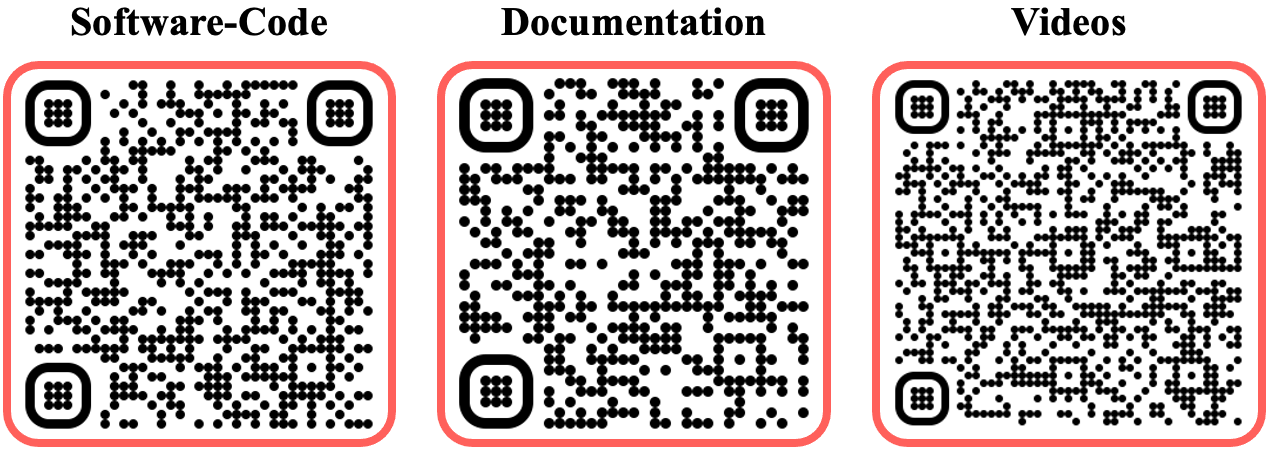
\includegraphics[width=0.79\textwidth]{qr_links}
    \caption[QR-Codes with links to sources]{QR-Codes with links to sources. The first code directs to the GitHub repository containing the source code, the second code to the repository containing the \LaTeX files to build this documentation, and the third code points to video visualisations of the results.}
    \figlbl{qr_links}
\end{figure}
%
The codebase and results from this thesis have been released as open source on GitHub: The code is available at \href{https://github.com/sagerpascal/lateral-connections}{github.com/sagerpascal/lateral-connections}, and the documentation is available at \href{https://github.com/sagerpascal/msc-thesis}{github.com/sagerpascal\\/msc-thesis}.
Furthermore, a GitHub webpage provides video visualisations from some of the results is available at \href{https://sagerpascal.github.io/lateral-connections/results/final_results.html}{sagerpascal.github.io/lateral-connections/results/final\_results}.
QR codes linking to these URLs are provided in \figref{qr_links} for convenient access using electronic devices.


\section{Video}\seclbl{result_video}
%
\begin{figure}[h]
    \centering
    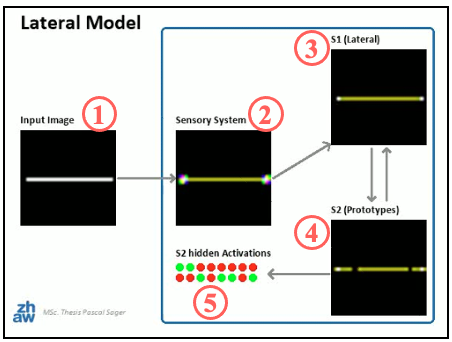
\includegraphics[width=0.99\textwidth]{video_overview}
    \caption[Overview of components visualised in the videos]{An overview of the components visualised in the videos.}
    \figlbl{video_overview}
\end{figure}
%
In the following, the video visualisations accessible at \href{https://sagerpascal.github.io/lateral-connections/results/final_results.html}{sagerpascal.github.io\\/lateral-connections/results/final\_results} are explained.
These explanations are limited to an overview of which components are shown in each video.
An interpretation of the video contents is provided in the corresponding result section.

Two video versions are shown for each experiment, both produced by the same model using the same parameter weights.
In the first video version, the Bernoulli neuron is replaced by a neuron using a fixed threshold.
This provides a video output that is more stable and has no flickering activations caused by sampling from a probability distribution.
For the \emph{S0} and \emph{S1} stages, a threshold of $0.5$ is used. Consequently, neurons with a probability of $\geq 0.5$ are set to $1$, while the other neurons are set to $0$.
A threshold of $0.9$ is used for the \emph{S2} stage, visualising only activities with high certainty that roughly correspond to those accepted by \emph{S1} as feedback signals.
The second video shows the network activities when the Bernoulli neurons are used.

Each video visualises the processing of the input over time.
The first six video frames show how the video is processed over the $T=6$ timesteps of the fast loop, followed by five additional frames depicting the final prediction after the fast loop.
By doing so, viewers have time to analyse the network's activations during this short interruption before the next input is fed into the model, and the process repeats.

\figref{video_overview} shows a single video frame, providing an overview of the components displayed in each video:
\begin{enumerate}
    \item The left part of the video displays the input image fed into the sensory system. It is a binary image with one colour channel, whereby active pixels are depicted in white and inactive pixels are depicted in black.
    \item The activations of the sensory system \emph{S0} are shown in the middle of the video. The sensory system extracts $4$ features at each location. Each feature combination is visualised in a different colour, and areas without activations are depicted in black.
    \item \emph{S1} is visualised in the top right corner. It uses the same colours as the sensory system. However, the activations might differ since neurons with insufficient lateral support are turned off, or other neurons might switch on.
    \item \emph{S2} is shown in the bottom right corner. It uses the same colours as the sensory system and \emph{L1}. The visualisation depicts the returned prototype, i.e., the feedback provided to \emph{S1} after mapping \emph{S1}' activities to the latent variables.
    \item The latent variables of \emph{S2} are shown at the center bottom of the video as $16$ circles. Each circle represents a cell, with green indicating an active cell and red indicating an inactive one. 
\end{enumerate}

For a detailed explanation of the content and observations in each video, please refer to the results chapter of this thesis.

\chapter{Negative Hebbian Learning}\chlbl{neg_hebb_updates}
%
\begin{figure}[h]
    \centering
    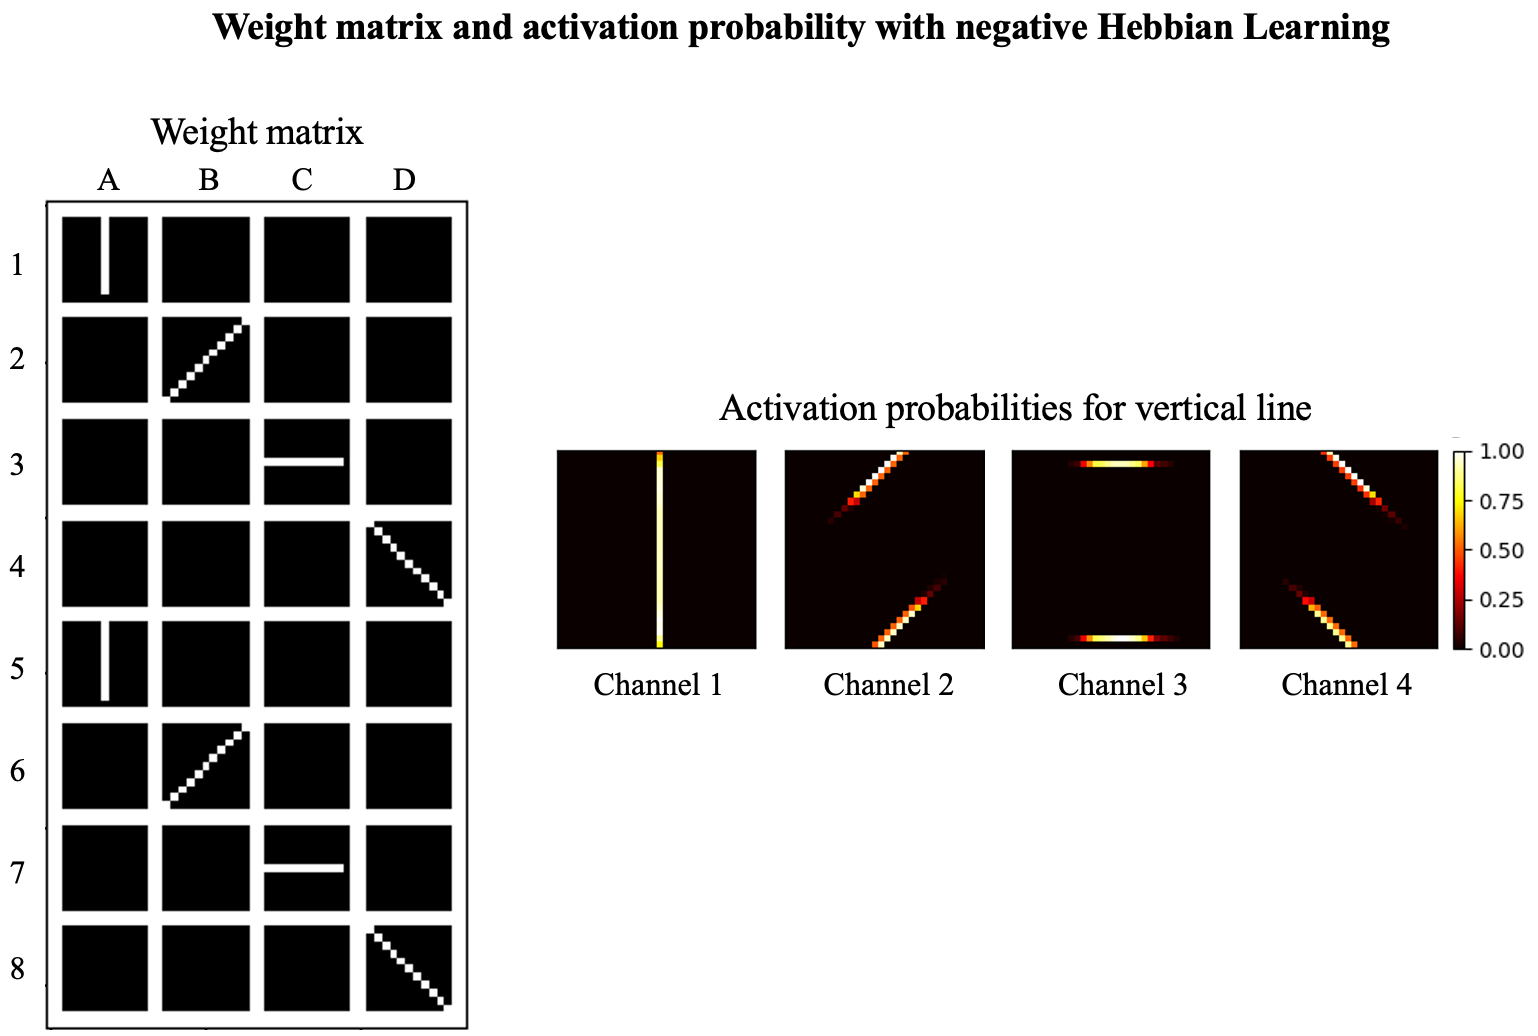
\includegraphics[width=0.99\textwidth]{neg_hebb_learning}
    \caption[Weight matrix and activations with negative Hebbian learning]{The weight matrix and the corresponding activation probabilities for a vertical line of a model trained with negative Hebbian learning.}
    \figlbl{neg_hebb_learning}
\end{figure}
%
This section examines the concept of negative Hebbian Learning in \emph{S1}, a learning paradigm designed to allow neural networks to forget unimportant or inconsistent features. 
In the conducted experiments, only positive Hebbian learning \sidecite{hebb_organization_1949} is used to strengthen connections between active cells.
Conversely, negative Hebbian learning additionally reduces the connection strength between cells that fire disjointly\sidenote{I.e. one cell is active while the other is inactive.}.
While negative Hebbian learning facilitates eliminating previously learned but inconsistent connections, it also poses challenges in maintaining desired lateral connections that are needed to provide support between feature cells.


\figref{neg_hebb_learning} visualises the weight matrix of a model trained with negative Hebbian updates and the activation probabilities if a vertical line fed is into the model.
Despite the divergence of the activation probabilities compared to those of positive Hebbian learning (c.f. \figref{S1_weight_analysis}), these activations are still considered valid representations of lines.
However, the major issue is that the output channels do not rely on multiple distinct features.

For instance, the output channel $A$ representing vertical lines only considers the input channels $1$ and $5$, whereby channel $1$ contains the ``vertical lines features'' from the sensory system, and channel $5$ is its own recurrent connection.
Regrettably, input channels $2$-$4$, which contain additional sensory signals, are disregarded by output channel $A$. Therefore, only cells representing vertical line features support this output channel.
In contrast, positive Hebbian learning considers all input channels, resulting in different features supporting each other.

Consequently, negative Hebbian learning leads to lower lateral support within the network.
This might not be an issue for the used line dataset but is crucial for real-world scenarios\sidenote{For example, one channel could represent eyes and another channel eyelashes. These features should support each other.}.
Negative Hebbian learning, while facilitating the filtering out of irrelevant features, also tends to make features mutually exclusive, which prevents learning adequate support between them.

\begin{figure}[h]
    \centering
    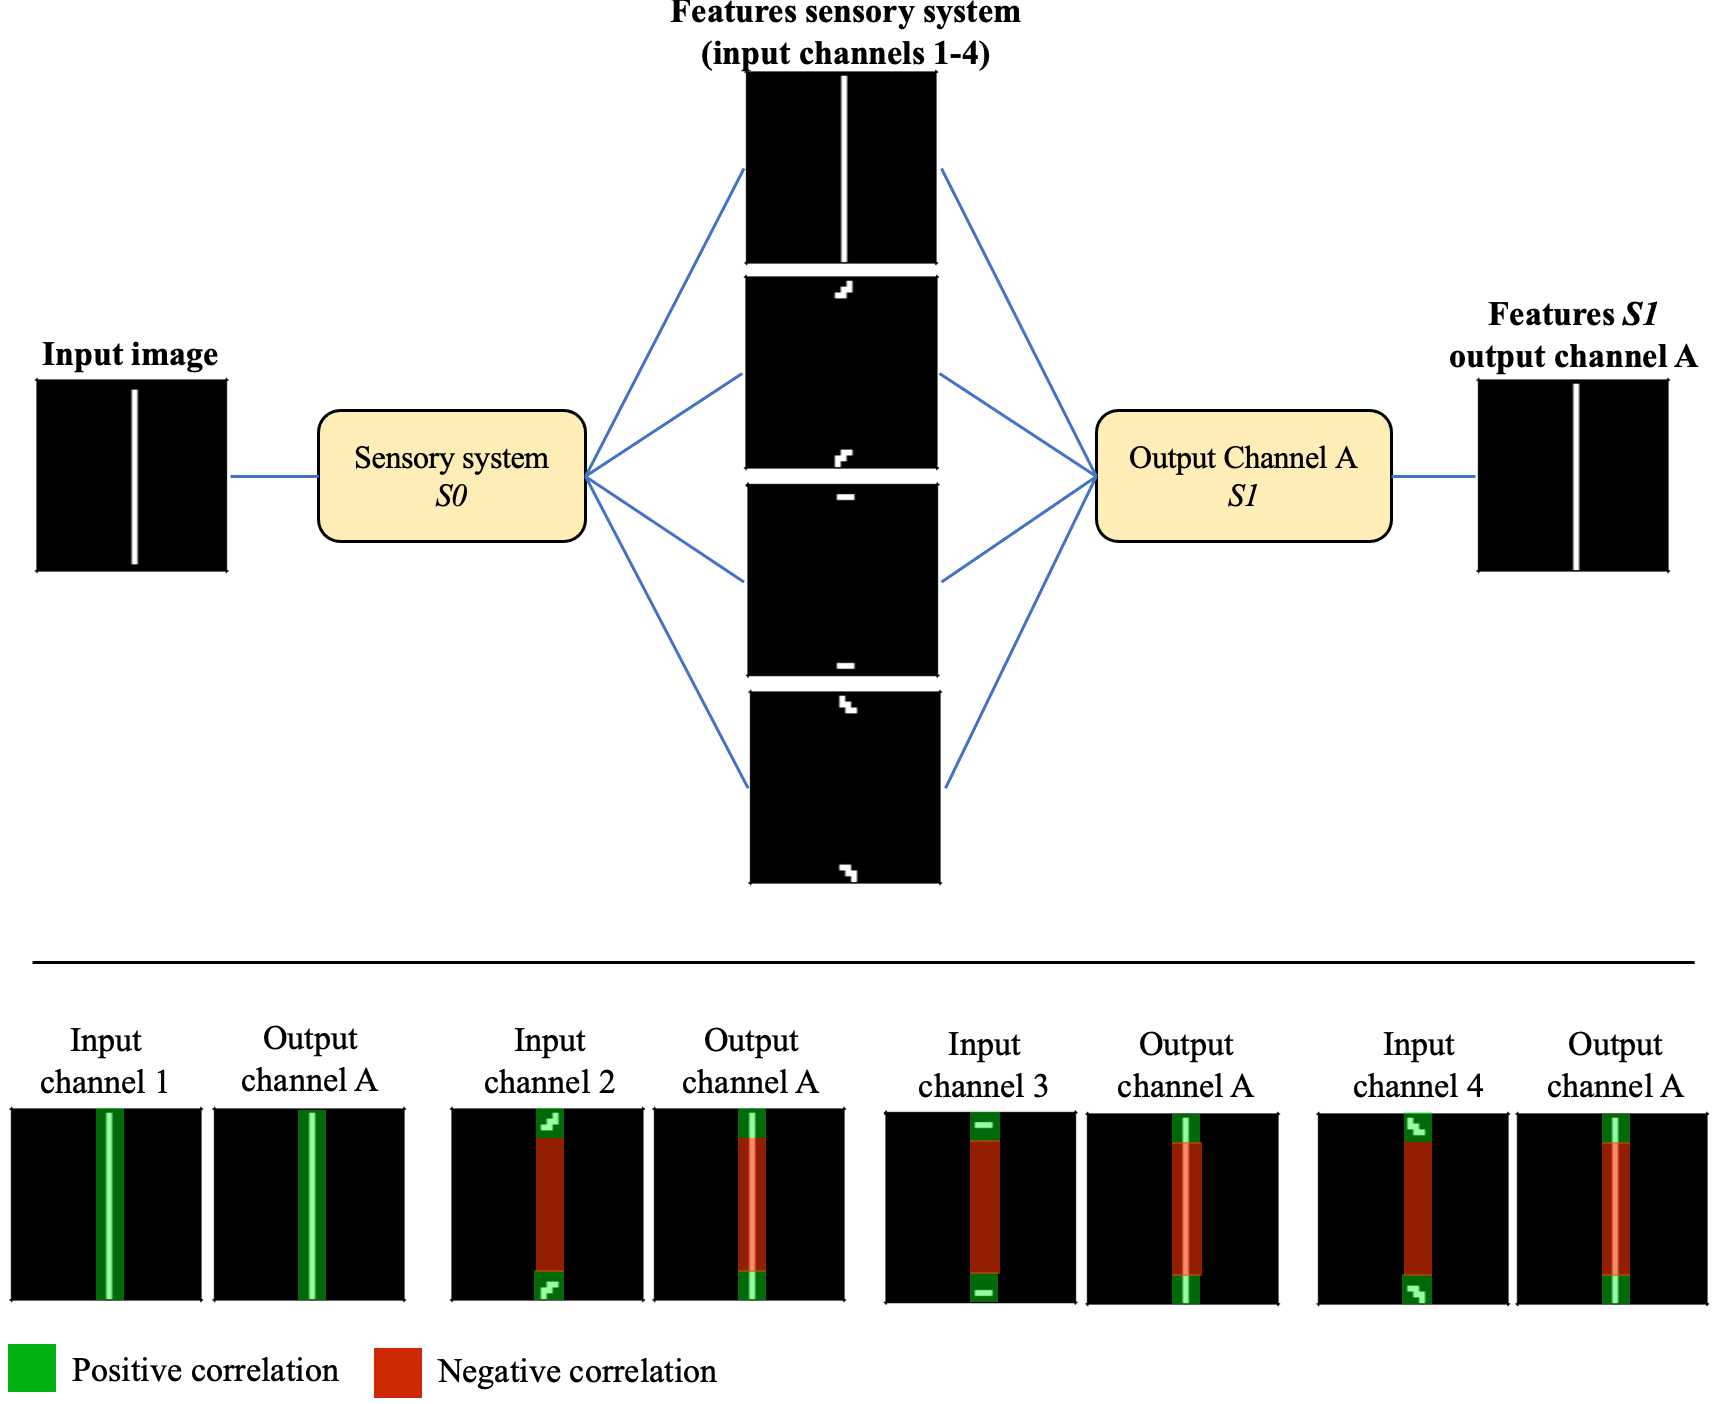
\includegraphics[width=0.99\textwidth]{correlations_hebb_learning}
    \caption[Feature correlation analysis]{Correlation between features from sensory input channels and the output channel $A$. The upper part of the images visualises the sensory features fed into output channel $A$ and the expected result. The lower part of the image indicates where positive and negative correlation occurs between sensory channels and output channel $A$.}
    \figlbl{correlations_hebb_learning}
\end{figure}
%
The primary issue is that, except for one input channel, there are more negative correlations between the input channels and a single output channel, as illustrated in \figref{correlations_hebb_learning}.
In this context, ``negative correlation'' refers to disjointly active cells, while ``positive correlation'' refers to cells that fire together.
In the case of the vertical line, the output channel $A$ is expected to reassemble the line roughly.

Hebbian learning compares this output with the input channels, strengthening the weights for positively correlated input-output pairs and weakening them for negatively correlated pairs.
These correlations are visualised in the lower part of \figref{correlations_hebb_learning}.
Input channel $1$ and output channel $A$ have high similarity. Therefore, the activations between input and output have a positive correlation, and the corresponding lateral connections undergo a positive Hebbian update.
However, all the other channels have a positive correlation only at the line ends and a negative correlation in the middle section of the line.
Consequently, there is more negative than positive correlation, and these features undergo more negative than positive updates.
This causes the lateral support learned at the line ends to be suppressed by the negative updates triggered by the negative correlation in the middle of the line.

The resolution to this issue remains unclear and requires additional experiments. One potential approach is to use a significantly lower learning rate for negative updates than for positive updates; another solution could be to introduce alternative cells (c.f. \secref{future_alt_cells})




%%%%%%%%%%%%%%%%%%%%%%%%%%%%%%%%%%%%%%%%%%%%%%%%%%%%%%%%%%%%%%%%%%%%%%%%%%%%%%%%
%%%%%%%%%%%%%%%%%%%%%%%%%%%%%%%%%%%%%%%%%%%%%%%%%%%%%%%%%%%%%%%%%%%%%%%%%%%%%%%%
\backmatter
\setchapterstyle{plain}


%%%%%%%%%%%%%%%%%%%%%%%%%%%%%%%%%%%%%%%%%%%%%%%%%%%%%%%%%%%%%%%%%%%%%%%%%%%%%%%%
\defbibnote{bibnote}{Here is the list of references in citation order.\par\bigskip}
\printbibliography[heading=bibintoc, title=Bibliography, prenote=bibnote]


%%%%%%%%%%%%%%%%%%%%%%%%%%%%%%%%%%%%%%%%%%%%%%%%%%%%%%%%%%%%%%%%%%%%%%%%%%%%%%%%
\printindex


%%%%%%%%%%%%%%%%%%%%%%%%%%%%%%%%%%%%%%%%%%%%%%%%%%%%%%%%%%%%%%%%%%%%%%%%%%%%%%%%
%\clearpage
%\thispagestyle{empty}
%\null%
%\clearpage
%\includepdf{cover-back.pdf}

%%%%%%%%%%%%%%%%%%%%%%%%%%%%%%%%%%%%%%%%%%%%%%%%%%%%%%%%%%%%%%%%%%%%%%%%%%%%%%%%
\end{document}
%%%%%%%%%%%%%%%%%%%%%%%%%%%%%%%%%%%%%%%%%%%%%%%%%%%%%%%%%%%%%%%%%%%%%%%%%%%%%%%%
